\documentclass[a4paper]{article}

\usepackage{inputenc}
\usepackage[british,UKenglish]{babel}
\usepackage{amsmath}
%\usepackage{titlesec}
\usepackage{color}
\usepackage{graphicx}
\usepackage{fancyref}
\usepackage{hyperref}
\usepackage{float}
\usepackage{scrextend}
\usepackage{setspace}
\usepackage{xargs}
\usepackage{multicol}
\usepackage{nameref}

\usepackage{sectsty}
\usepackage{multicol}
\usepackage{multirow}
\usepackage[procnames]{listings}
\usepackage{appendix}

\newcommand\tab[1][1cm]{\hspace*{#1}}
\hypersetup{colorlinks=true, linkcolor=black}
\interfootnotelinepenalty=10000

\newcommand{\cleancode}[1]{\begin{addmargin}[3em]{3em}\texttt{\textcolor{cleanOrange}{#1}}\end{addmargin}}
\newcommand{\cleanstyle}[1]{\text{\textcolor{cleanOrange}{\texttt{#1}}}}


\usepackage[colorinlistoftodos,prependcaption,textsize=footnotesize]{todonotes}
\newcommandx{\commred}[2][1=]{\textcolor{Red}
{\todo[linecolor=red,backgroundcolor=red!25,bordercolor=red,#1]{#2}}}
\newcommandx{\commblue}[2][1=]{\textcolor{Blue}
{\todo[linecolor=blue,backgroundcolor=blue!25,bordercolor=blue,#1]{#2}}}
\newcommandx{\commgreen}[2][1=]{\textcolor{OliveGreen}{\todo[linecolor=OliveGreen,backgroundcolor=OliveGreen!25,bordercolor=OliveGreen,#1]{#2}}}
\newcommandx{\commpurp}[2][1=]{\textcolor{Plum}{\todo[linecolor=Plum,backgroundcolor=Plum!25,bordercolor=Plum,#1]{#2}}}

\def\code#1{{\tt #1}}

\def\note#1{\noindent{\bf [Note: #1]}}

\makeatletter
%% The "\@seccntformat" command is an auxiliary command
%% (see pp. 26f. of 'The LaTeX Companion,' 2nd. ed.)
\def\@seccntformat#1{\@ifundefined{#1@cntformat}%
   {\csname the#1\endcsname\quad}  % default
   {\csname #1@cntformat\endcsname}% enable individual control
}
\let\oldappendix\appendix %% save current definition of \appendix
\renewcommand\appendix{%
    \oldappendix
    \newcommand{\section@cntformat}{\appendixname~\thesection\quad}
}
\makeatother


% "define" Scala
\usepackage[T1]{fontenc}  
\usepackage[scaled=0.82]{beramono}  
\usepackage{microtype} 

\sbox0{\small\ttfamily A}
\edef\mybasewidth{\the\wd0 }

\lstdefinelanguage{scala}{
  morekeywords={abstract,case,catch,class,def,%
    do,else,extends,false,final,finally,%
    for,if,implicit,import,match,mixin,%
    new,null,object,override,package,%
    private,protected,requires,return,sealed,%
    super,this,throw,trait,true,try,%
    type,val,var,while,with,yield},
  sensitive=true,
  morecomment=[l]{//},
  morecomment=[n]{/*}{*/},
  morestring=[b]",
  morestring=[b]',
  morestring=[b]"""
}

\usepackage{color}
\definecolor{dkgreen}{rgb}{0,0.6,0}
\definecolor{gray}{rgb}{0.5,0.5,0.5}
\definecolor{mauve}{rgb}{0.58,0,0.82}

% Default settings for code listings
\lstset{frame=tb,
  language=scala,
  aboveskip=3mm,
  belowskip=3mm,
  showstringspaces=false,
  columns=fixed, % basewidth=\mybasewidth,
  basicstyle={\small\ttfamily},
  numbers=none,
  numberstyle=\footnotesize\color{gray},
  % identifierstyle=\color{red},
  keywordstyle=\color{blue},
  commentstyle=\color{dkgreen},
  stringstyle=\color{mauve},
  frame=single,
  breaklines=true,
  breakatwhitespace=true,
  procnamekeys={def, val, var, class, trait, object, extends},
  procnamestyle=\ttfamily\color{red},
  tabsize=2
}

\lstnewenvironment{scala}[1][]
{\lstset{language=scala,#1}}
{}
\lstnewenvironment{cpp}[1][]
{\lstset{language=C++,#1}}
{}
\lstnewenvironment{bash}[1][]
{\lstset{language=bash,#1}}
{}
\lstnewenvironment{verilog}[1][]
{\lstset{language=verilog,#1}}
{}



%代码段设置
\lstset{numbers=left,
basicstyle=\tiny,
numberstyle=\tiny,
keywordstyle=\color{blue!70},
commentstyle=\color{red!50!green!50!blue!50},
frame=single, rulesepcolor=\color{red!20!green!20!blue!20},
escapeinside=``
}

\graphicspath{ {images/} }
\usepackage{ctex}
\usepackage{graphicx}
\usepackage{color,framed}%文本框
\usepackage{listings}
\usepackage{caption}
\usepackage{amssymb}
\usepackage{enumerate}
\usepackage{xcolor}
\usepackage{bm} 
\usepackage{lastpage}%获得总页数
\usepackage{fancyhdr}
\usepackage{tabularx}  
\usepackage{geometry}
\usepackage{minted}
\usepackage{graphics}
\usepackage{subfigure}
\usepackage{float}
\usepackage{pdfpages}
\usepackage{pgfplots}
\pgfplotsset{width=10cm,compat=1.9}
\usepackage{multirow}
\usepackage{footnote}
\usepackage{booktabs}

%-----------------------伪代码------------------
\usepackage{algorithm}  
\usepackage{algorithmicx}  
\usepackage{algpseudocode}  
\floatname{algorithm}{Algorithm}  
\renewcommand{\algorithmicrequire}{\textbf{Input:}}  
\renewcommand{\algorithmicensure}{\textbf{Output:}} 
\usepackage{lipsum}  
\makeatletter
\newenvironment{breakablealgorithm}
  {% \begin{breakablealgorithm}
  \begin{center}
     \refstepcounter{algorithm}% New algorithm
     \hrule height.8pt depth0pt \kern2pt% \@fs@pre for \@fs@ruled
     \renewcommand{\caption}[2][\relax]{% Make a new \caption
      {\raggedright\textbf{\ALG@name~\thealgorithm} ##2\par}%
      \ifx\relax##1\relax % #1 is \relax
         \addcontentsline{loa}{algorithm}{\protect\numberline{\thealgorithm}##2}%
      \else % #1 is not \relax
         \addcontentsline{loa}{algorithm}{\protect\numberline{\thealgorithm}##1}%
      \fi
      \kern2pt\hrule\kern2pt
     }
  }{% \end{breakablealgorithm}
     \kern2pt\hrule\relax% \@fs@post for \@fs@ruled
  \end{center}
  }
\makeatother
%------------------------代码-------------------
\usepackage{xcolor} 
\usepackage{listings} 
\lstset{ 
breaklines,%自动换行
basicstyle=\small,
escapeinside=``,
keywordstyle=\color{ blue!70} \bfseries,
commentstyle=\color{red!50!green!50!blue!50},% 
stringstyle=\ttfamily,% 
extendedchars=false,% 
linewidth=\textwidth,% 
numbers=left,% 
numberstyle=\tiny \color{blue!50},% 
frame=trbl% 
rulesepcolor= \color{ red!20!green!20!blue!20} 
}

%-------------------------页面边距--------------
\geometry{a4paper,left=2.3cm,right=2.3cm,top=2.7cm,bottom=2.7cm}
%-------------------------页眉页脚--------------
\usepackage{fancyhdr}
\pagestyle{fancy}
\lhead{\kaishu \leftmark}
% \chead{}
\rhead{\kaishu 并行程序设计实验报告}%加粗\bfseries 
\lfoot{}
\cfoot{\thepage}
\rfoot{}
\renewcommand{\headrulewidth}{0.1pt}  
\renewcommand{\footrulewidth}{0pt}%去掉横线
\newcommand{\HRule}{\rule{\linewidth}{0.5mm}}%标题横线
\newcommand{\HRulegrossa}{\rule{\linewidth}{1.2mm}}
\setlength{\textfloatsep}{10mm}%设置图片的前后间距
%--------------------文档内容--------------------

\begin{document}
\renewcommand{\contentsname}{目\ 录}
\renewcommand{\appendixname}{附录}
\renewcommand{\appendixpagename}{附录}
\renewcommand{\refname}{参考文献} 
\renewcommand{\figurename}{图}
\renewcommand{\tablename}{表}
\renewcommand{\today}{\number\year 年 \number\month 月 \number\day 日}

%-------------------------封面----------------
\begin{titlepage}
    \begin{center}
    
\includegraphics[width=0.8\textwidth]{NKU.png}\\[1cm]
    \vspace{20mm}
		\textbf{\huge\textbf{\kaishu{计算机学院}}}\\[0.5cm]
		\textbf{\huge{\kaishu{并行程序设计开题报告}}}\\[2.3cm]
		\textbf{\Huge\textbf{\kaishu{并行加速的高斯消去算法}}}

		\vspace{\fill}
    
    % \textbf{\Large \textbf{并行程序设计期末实验报告}}\\[0.8cm]
    % \HRule \\[0.9cm]
    % \HRule \\[2.0cm]
    \centering
    \textsc{\LARGE \kaishu{姓名\ :\ 熊宇轩}}\\[0.5cm]
    \textsc{\LARGE \kaishu{学号\ :\ 2010056}}\\[0.5cm]
    \textsc{\LARGE \kaishu{专业\ :\ 计算机科学与技术}}\\[0.5cm]
    
    \vfill
    {\Large \today}
    \end{center}
\end{titlepage}

\renewcommand {\thefigure}{\thesection{}.\arabic{figure}}%图片按章标号
\renewcommand{\figurename}{图}
\renewcommand{\contentsname}{目录}  
\cfoot{\thepage\ of \pageref{LastPage}}%当前页 of 总页数


% 生成目录
\clearpage
\tableofcontents
\newpage

%--------------------------Title--------------------------------


\section{研究问题描述}
\subsection{普通高斯消去}
高斯消去,是线性代数的一个算法,用于将矩阵转化为行阶梯形矩阵。高斯消去可用来进行线性方程组求解,矩阵求秩,以及逆矩阵的计算。



高斯消去的典型串行算法具体步骤如下:


\begin{enumerate}
  \item 读入一个$N*N$的矩阵,设置变量$i=0$代表当前正在处理的行
  \item 通过行变换的方法,用第$i$行去消除$i+1$到$N$行的第$i$个元素。使得矩阵的$i$列中,$i$行以下的元素全为0
  \item $i$自增, 若$i>N$,则消元结束。
\end{enumerate}



其对应的伪代码如下


\begin{minted}[mathescape,
               linenos,
               numbersep=5pt,
               gobble=2,
               frame=lines,
               framesep=2mm,
               highlightcolor=green!40]{python}

    def LU(matrix):
        N = len(matrix)
        for i in range(N): # 遍历矩阵行
            for j in range(i+1, N): # 遍历i以下的行
                divisor = matrix[j][i] / matrix[i][i] # 被除数
                for k in range(i,N): # 遍历j行i列到N列的元素
                    matrix[j][k] -= matrix[i][k] * divisor
        return matrix
\end{minted}

不难发现,普通高斯消去算法包含着一个三重循环,总的循环执行的步数为$N*\frac{n}{2}*\frac{n}{2} = \frac{n^{3}}{4}$,因此算法的时间复杂度为$O(n^{3})$。


\subsection{Gröbner基计算中的高斯消去}
Gröbner基是一组多变量非线性多项式,而其所具有的某些特性,可以为数学、自然科学和计算机科学中的许多基本问题提供简单的算法解决方案,在密码学中,其可以被应用于公钥密码、数字签名和零知识证明等领域。而在Gröbner基生成算法中,多项式所产生的矩阵多为大型稀疏矩阵,而约化这些大型矩阵的过程,则可以通过$GF(2)$上的特殊高斯消去算法来完成。\cite{狄鹏2008Grobner}

$GF(2)$上的特殊高斯消去算法和普通高斯消去算法主要有以下几点不同:

\begin{enumerate}
  \item 输入矩阵中的元素全部都是有限域$GF(2)$上的元素,也就是说,矩阵中只含有0和1两种元素。
  \item 矩阵行变换过程中也需要遵守有限域$GF(2)$的运算规则,而在有限域$GF(2)$上,加减法是等同于异或运算的。
  \item 特殊高斯消去算法将矩阵行分为了两类——“消元子”和“被消元行”。消元子行可以被填入一个矩阵中,这个矩阵可能具有空行,但是可以保证所有消元子的首个非零元素处于该矩阵的对角线上,且不会出现消元子冲突的情况(可以保证消元子的首行非零元的位置都不同)。被消元行则充当消元过程中的“被减数”,但被消元行也有可能因为找不到对应的消元子而被升格为消元子。
\end{enumerate}

其串行算法的过程如下:

\begin{enumerate}
    \item 如果待处理的数据规模过大,可能需要将消元子和被消元行分批次读入内存。
    \item 对于当前批次中的所有被消元行,检查其首项,并用对应的消元子将其首项目消去,重复执行此过程,直到该行全为0,或者其需要的消元子不在当前批次内,或者没有其首项对应的消元子。对于第一种情况,将该行丢弃,而对于第三种情况,则将该被消元行升格为消元子。
    \item 当该批次处理完后,读入下一批次消元子,当所有消元子都被使用过后,读入下一次批次被消元行。如此重复,直到得到最终结果
\end{enumerate}



\section{前人工作总结}

查阅资料得知,可供参考的前人在高斯消去算法上得到的的加速成果主要有以下四个:

\begin{itemize}
    \item 刘琳在2011年描述的用于对称方程组系数矩阵的并行高斯消去算法\cite{lin_liu_song_2011}
    \item Simplice Donfack等人于2014年对5种高斯消去算法的介绍与比较\cite{donfack2015survey}
    \item Jean Charles于2010年实现的用于Gröbner基计算的并行化高斯消去算法\cite{faugere2010parallel}
    \item Mark Hojnacki等人于2021年在NVIDIA GPU上通过CUDA实现的用于Gröbner基计算的高斯消去算法\cite{hojnacki2021parallel}
\end{itemize}

其中,刘琳等人描述的用于对角线对称矩阵的普通高斯消去算法是最为简单的并行方法,除了通过矩阵对称性节约存储空间外,还通过“卷帘法”进行了并行任务划分。具体来说,就是让每个节点处理所有行数为$procid+nprocs*x (x \in \mathbb{Z})$的行。之所以要这么做,是因为如果单纯的按行平均的划分任务,节点分配到的行越靠上,所需要计算的次数就越少,于是就会造成任务的不平衡。

\begin{table}[!htbp]
    \centering
    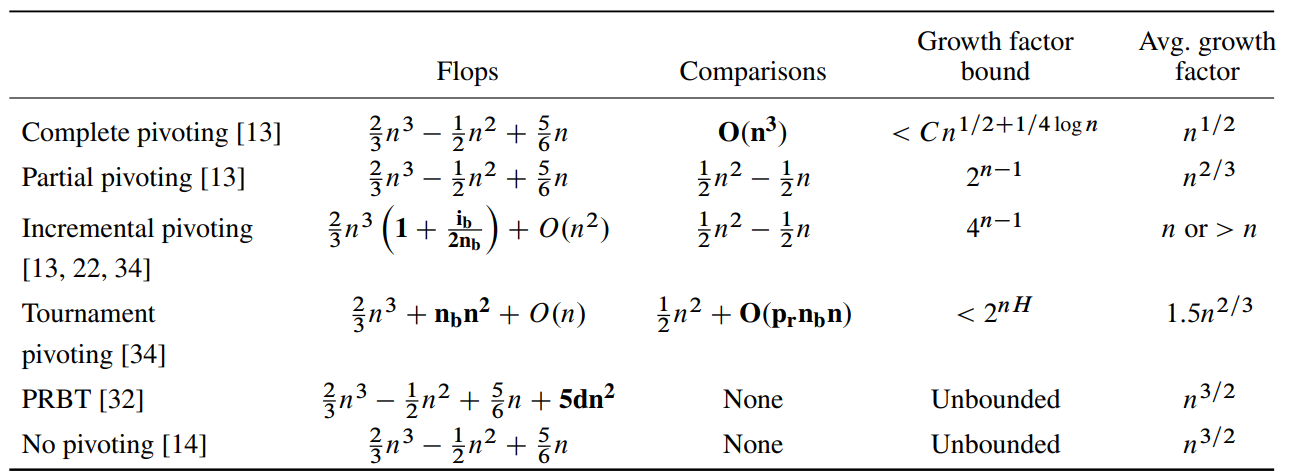
\includegraphics[width=6in]{fig/pivoting.png}
    \caption{几种不同的Pivoting策略性能比较}
    \label{tab:pivoting}
\end{table}

在高斯消去的并行化过程中,寻找主元(pivoting)的策略是极为关键的。Simplice Donfack等人则对几种具有不同的主元寻找方法的并行化算法进行了介绍、复杂度分析和性能比较。表\ref{tab:pivoting}是他们比较得出的结果。

Jean Charles提出的并行Gröbner基计算算法的大致思想,则是将输入矩阵进行划分,分为四个来自主元和非主元行和列的子矩阵,之后再进行计算。其大致过程如下:\cite{faugere2010parallel}

\begin{equation}
    M_{0} \sim\left(\begin{array}{c|c}
I d & A^{-1} B \\
\hline C & D
\end{array}\right)
\end{equation}

\begin{equation}
M_{0} \sim\left(\begin{array}{c|c}
I d & A^{-1} B \\
\hline 0 & D-C A^{-1} B
\end{array}\right)
\end{equation}

\begin{equation}
M_{0} \sim\left(\begin{array}{c|c}
I d & A^{-1} B \\
\hline 0 & \operatorname{Gauss}\left(D-C A^{-1} B\right)
\end{array}\right)
\end{equation}

\begin{figure}[!htbp]
    \centering
    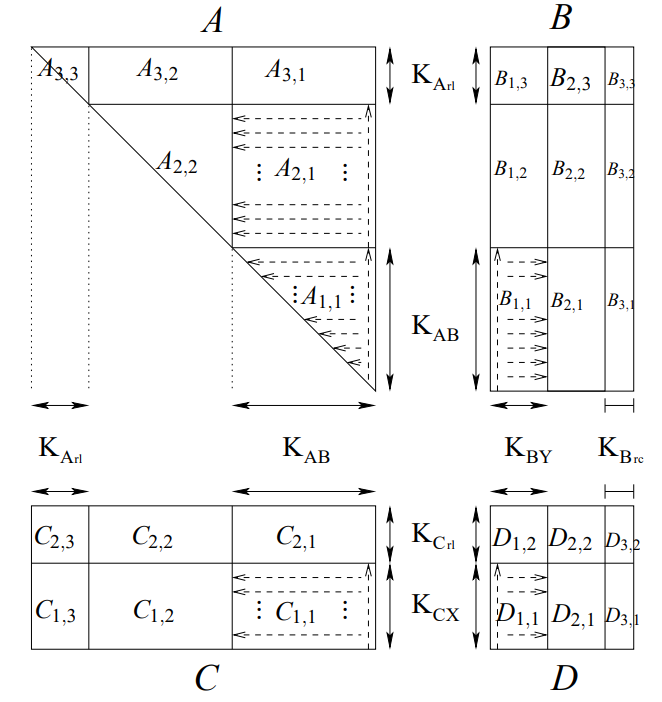
\includegraphics[width=3.2in]{fig/screenshot-20220405-143249.png}
    \caption{Jean Charles所提出的并行加速算法中的矩阵划分与分块\cite{faugere2010parallel}}
    \label{fig:matrices_partrition}
\end{figure}

相较于之前其他针对F4、F5算法的并行加速方法,Jean Charles所提出的并行加速算法在数据结构方面考虑了如何充分利用现代CPU中的缓存。如图\ref{fig:matrices_partrition}所示该算法为了尽可能多地从缓存中获益,将每个矩阵都分割成了小块。

此外,Joan Charles还区分了三种子矩阵的存储方式:稀疏三角块、稀疏矩形块和混合矩形块。而实际的存储方式可以在运算过程中变化,以适应经过多次运算后变得稠密的矩阵。\cite{faugere2010parallel}

\begin{table}[!htbp]
    \centering
    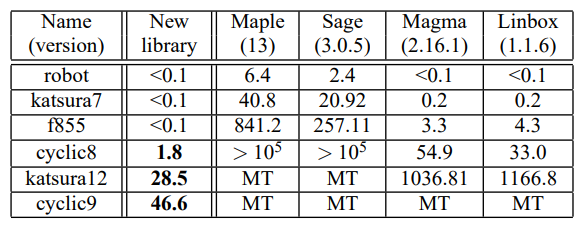
\includegraphics[width=4.8in]{fig/f4time.png}
    \caption{Jean Charles所提出的并行加速算法与其他线性代数库在标准测试中所使用的时间\cite{faugere2010parallel}}
    \label{tab:f4benchmark}
\end{table}

从表\ref{tab:f4benchmark}中可以看到,在2010年时Joan Charles的并行库相较于其他并行线性代数库性能优化显著。

\begin{table}[!htbp]
    \centering
    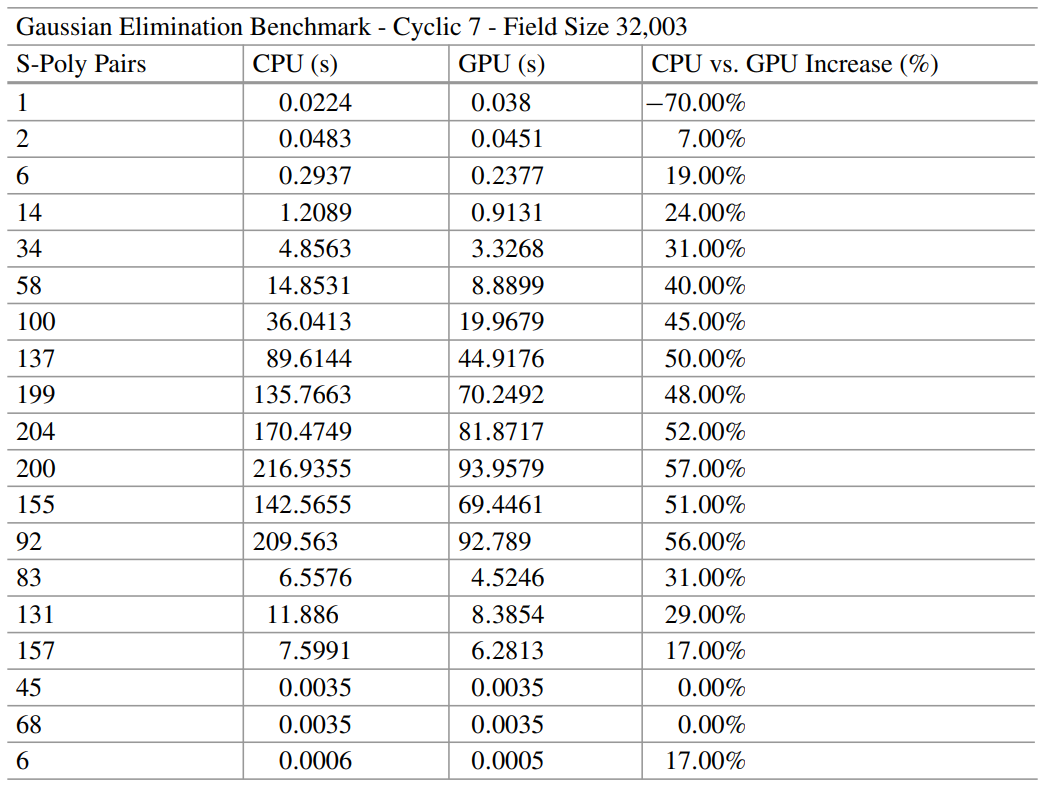
\includegraphics[width=5.4in]{fig/cuda.png}
    \caption{Jean Charles所提出的并行加速算法与其他线性代数库在标准测试中所使用的时间\cite{faugere2010parallel}}
    \label{tab:cudabenchmark}
\end{table}

高斯消去作为一个计算密集型任务,自然可以使用GPU进行加速,Mark Hojnacki等人于2021年在NVIDIA GPU上通过CUDA实现了加速的F4/F5算法。如图\ref{tab:cudabenchmark}所示,他们的算法在标准测试中获得了一定的加速比。





\section{研究方案}

\subsection{研究问题及思路}

Gröbner基计算中的高斯消去所处理的矩阵大多为稀疏矩阵,按照位向量存储可能会导致一定的空间浪费。我们可以采用三元组、倒排链表的方式进行压缩存储,但是这样也会增加算法的复杂性和并行化的难度。这个问题是一个需要权衡利弊的值得探讨的问题。

此外,对于多项式生成的对称矩阵,其也具有在高斯消去过程中保持对称的特性,因此我们也可以在数据结构上进行一定的优化。\cite{lin_liu_song_2011}

高斯消去的并行化还包含了一个重要内容——pivoting策略的选取,如表\ref{tab:f4benchmark}所示,不同的pivoting策略对于不同的输入数据规模所获得的加速比肯定都是不一样的,而这些pivoting策略在arm和X86平台上可能也会出现性能的差异,这是一个值得研究的问题。不过实现五个pivoting策略确实有一定的难度,如果时间不允许,选取几个有代表性的策略进行测试可能是比较好的解决方法。

此外,当我们遇到规模较大,无法存入全部内存的数据,我们还需要考虑算法中外存访问的相关内容。除了对矩阵进行分批读取外,计算和访存异步模式也是可以考虑的方法之一。

由于对GPU编程还不是很熟悉,我暂时还没有决定是通过oneAPI和CUDA来进行GPU并行加速的实现,但是前人工作中可以找到相关的实现思路。\cite{hojnacki2021parallel}

\subsection{研究计划}
结合上文中提出的研究问题及思路、课程内容和前人研究,列出研究的任务清单如下:
% Please add the following required packages to your document preamble:
% \usepackage{booktabs}
\begin{table}[!htbp]
\centering
\begin{tabular}{@{}ll@{}}
\toprule
时间节点 & 任务                                  \\ \midrule
第8周  & 完成普通高斯消去的串行算法和ARM平台SIMD加速           \\
第8周  & 完成Gröbner基计算中的高斯消去的串行算法和ARM平台SIMD加速 \\
第9周  & 进行两种高斯消去算法SIMD加速在X86和ARM两种不同平台上的比较  \\
第10周 & 通过Pthread和OpenMP实现多核加速的两种高斯消去算法     \\
第10周 & 对Gröbner基计算中的高斯消去算法的数据结构进行研究     \\
第12周 & 通过MPI实现集群加速的两种高斯消去算法                \\
第12周 & 验证高斯消去不同Pivoting策略在不同平台上对性能的影响                \\
第13周 & 尝试对高斯消去的外存访存进行优化                \\
第14周 & 通过oneAPI或CUDA编程实现GPU加速的两种高斯消去算法     \\
第15周 & 进一步优化、整理成果、探索加速算法的具体应用场景                          \\ \bottomrule
\end{tabular}
\end{table}

\subsection{总结}
由于这学期课业比较繁重,且需要在两校区之间往返,再加上之前对并行程序设计没有了解,因此任务的完成度可能会有一定折扣。但相信只要尽力开展了研究,所学到的知识,积累的经验都会是非常丰富的。








\newpage
\bibliographystyle{plain}
\bibliography{reference.bib} 

\end{document}